\section{Configurazione iniziale del progetto}
\subsection{Spring Initializr}

\begin{figure}[!h] 
    \centering 
    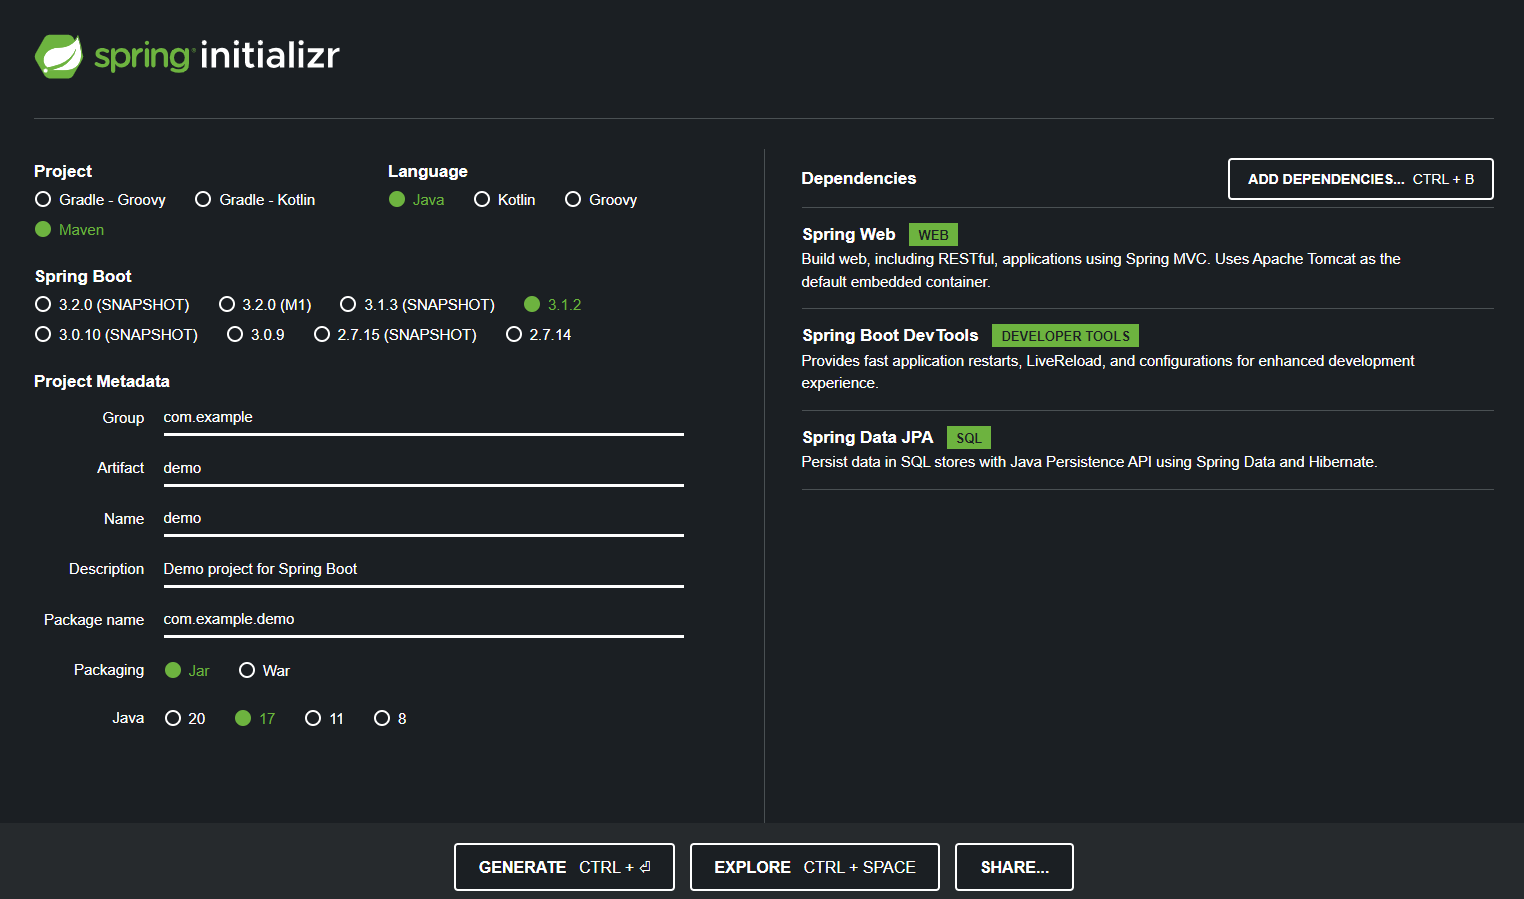
\includegraphics[width=0.95\columnwidth]{Spring_initializr} 
    \caption{Interfaccia Spring Initializr}
\end{figure}

\noindent \href{https://start.spring.io/}{Spring Initializr} è uno strumento online fornito dalla community di Spring Framework, che consente di creare rapidamente un progetto Spring Boot personalizzato, con le dipendenze e le configurazioni preselezionate dall'utente. Questo strumento semplifica notevolmente il processo di inizializzazione di un progetto Spring Boot, permettendo agli sviluppatori di risparmiare tempo e concentrarsi sulla scrittura del codice.\\
L'utente può selezionare il tipo di progetto di cui ha bisogno, come ad esempio un progetto Maven o Gradle, e specificare il linguaggio e la versione di Spring Boot desiderati. Inoltre, può anche inserire i metadati del progetto, come il nome del progetto e il nome dei packages.\\
Una volta selezionate le opzioni desiderate, l'utente può scegliere le dipendenze per il progetto. Le dipendenze sono librerie di terze parti che forniscono funzionalità aggiuntive al progetto.\\
Dopo aver selezionato le dipendenze, l'utente può scaricare il progetto Spring Boot personalizzato in formato ZIP. 

\subsection{Contenuto del pacchetto}
Il file ZIP scaricato precedentemente contiene tutti i file necessari per iniziare a lavorare sul progetto. All'interno di questo pacchetto troviamo i seguenti elementi rilevanti:
\begin{itemize}
\item file di configurazione \textit{application.properties} e file di build \textit{pom.xml} con le dipendenze selezionate;
\item classe principale, rappresenta il punto di ingresso dell'applicazione ed è annotata con \textit{@SpringBootApplication}. Il metodo \texttt{main()} al suo interno avvierà l'applicazione Spring;
\item una struttura base dei package.
\end{itemize}
Di seguito riporto uno snippet\textsubscript{g} del file di build \textit{pom.xml} che si ottiene creando un progetto con le dipendenze sopra selezionate. La configurazione di Maven avviene proprio tramite questo file.\\
All'interno di questo file si possono trovare i seguenti tag:
\begin{itemize}
\item \textit{<dependecies>}, indica una lista di dipendenze;
\item \textit{<build>}, contiene impostazioni di costruzione e compilazione;
\item \textit{<plugins>}, contiene plugin di Maven;
\item \textit{<properties>}, contiene proprietà definite dall'utente;
\item \textit{<groupId>}, organizzazione che ha creato il progetto;
\item \textit{<artifactId>}, nome unico del progetto;
\item \textit{<version>},  versione del progetto.
\end{itemize}

\noindent Nel file si possono notare le seguenti dipendenze:
\begin{itemize}
\item \textit{spring-boot-starter-web}, per utilizzare il framework Spring MVC per la creazione di applicazioni Web;
\item \textit{spring-boot-starter-jpa}, per la persistenza dei dati;
\item \textit{spring-boot-devtools}, offre tools per migliorare il processo di sviluppo come live reload e rilascio automatico;
\item \textit{spring-boot-starter-test}, per includere librerie di testing.
\end{itemize}
Rispetto al file utilizzato nel progetto mancano le seguenti dipendenze:
\begin{itemize}
\item \textit{Dipendenza 1};
\item \textit{Dipendenza 2};
\item \textit{Dipendenza 3}.
\end{itemize}
\begin{figure}[H] 
    \centering 
    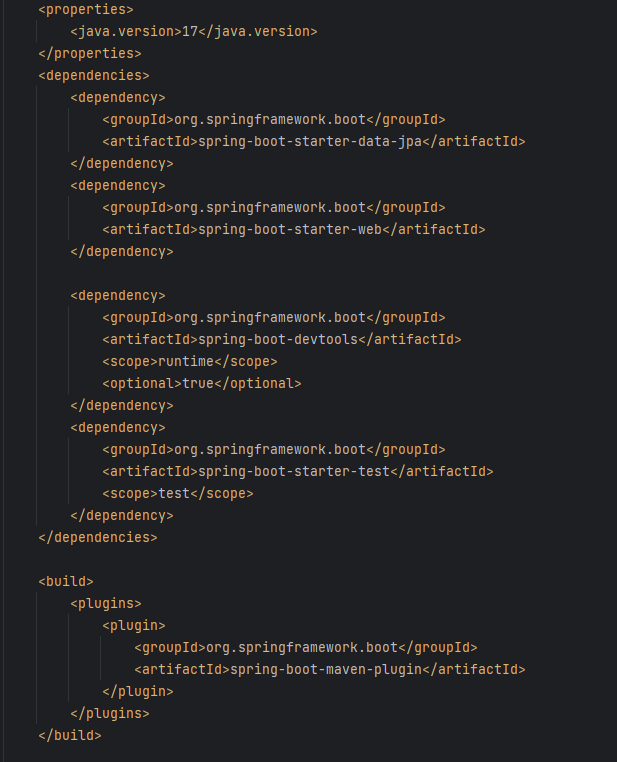
\includegraphics[width=0.85\columnwidth]{foto_pom_base} 
    \caption{Snippet pom.xml generato}
\end{figure}
%\begin{lstlisting}[language=XML,caption = pom.xml con dipendenze selezionate]
%	<properties>
%		<java.version>17</java.version>
%	</properties>
%	<dependencies>
%		<dependency>
%			<groupId>org.springframework.boot</groupId>
%			<artifactId>spring-boot-starter-data-jpa</artifactId>
%		</dependency>
%		<dependency>
%			<groupId>org.springframework.boot</groupId>
%			<artifactId>spring-boot-starter-web</artifactId>
%		</dependency>
%
%		<dependency>
%			<groupId>org.springframework.boot</groupId>
%			<artifactId>spring-boot-devtools</artifactId>
%			<scope>runtime</scope>
%			<optional>true</optional>
%		</dependency>
%		<dependency>
%			<groupId>org.springframework.boot</groupId>
%			<artifactId>spring-boot-starter-test</artifactId>
%			<scope>test</scope>
%		</dependency>
%	</dependencies>
%
%	<build>
%		<plugins>
%			<plugin>
%				<groupId>org.springframework.boot</groupId>
%				<artifactId>spring-boot-maven-plugin</artifactId>
%			</plugin>
%		</plugins>
%	</build>
%
%\end{lstlisting}

\noindent Il secondo file qui sotto rappresentato è il file configurazione \textit{application.properties}. Di seguito riporto il file che ho utilizzato nel progetto:
\begin{figure}[H] 
    \centering 
    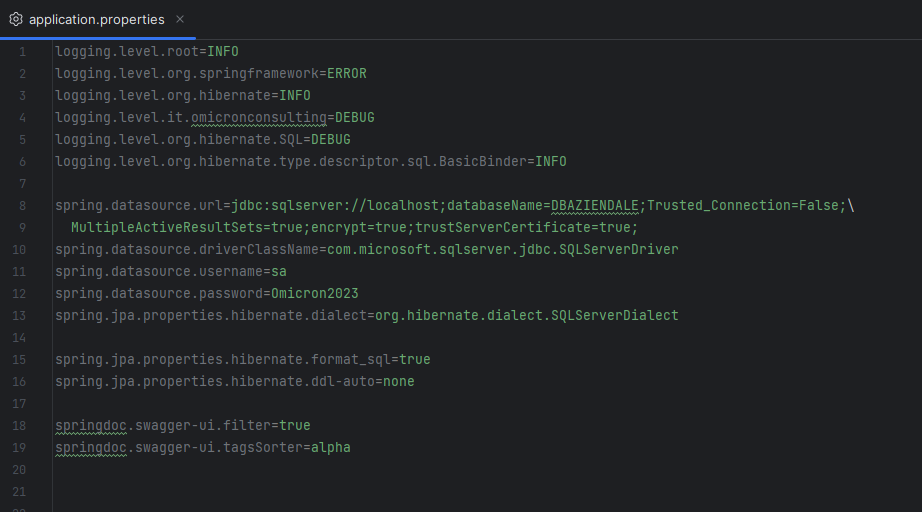
\includegraphics[width=0.85\columnwidth]{foto_application_properties} 
    \caption{Foto application.properties configurato e utilizzato}
\end{figure}
%\begin{lstlisting}[language = XML, caption = application.properties del progetto]
%logging.level.root=INFO
%logging.level.org.springframework=ERROR
%logging.level.org.hibernate=TRACE
%logging.level.it.omicronconsulting=DEBUG
%logging.level.org.hibernate.SQL=DEBUG
%logging.level.org.hibernate.type.descriptor.sql.BasicBinder=TRACE
%
%
%spring.datasource.url=jdbc:sqlserver://localhost;databaseName=DBDELIVERONE;Trusted_Connection=False;\MultipleActiveResultSets=true;encrypt=true;trustServerCertificate=true;
%spring.datasource.driverClassName=com.microsoft.sqlserver.jdbc.SQLServerDriver
%spring.datasource.username=SA
%spring.datasource.password=Password.1
%
%
%spring.jpa.properties.hibernate.format_sql=true
%spring.jpa.hibernate.dialect=org.hibernate.dialect.SQLServerDialect
%spring.jpa.hibernate.ddl-auto=validate
%
%springdoc.swagger-ui.filter=true
%springdoc.swagger-ui.tagsSorter=alpha
%\end{lstlisting}
Possiamo notare come il file utilizzi un formato di configurazione basato su chiavi e valori. Le chiavi rappresentano le diverse proprietà di configurazione dell'applicazione, mentre i valori rappresentano le impostazioni specifiche.\\
Nel file possiamo notare le seguenti chaivi:
\begin{itemize}
\item \textit{logging.level}, servono per configurare il livello di dettaglio dei log per diverse classi o package all'interno dell'applicazione;
\item \textit{spring.datasource}, servono per collegarsi ad un database, in questo caso locale, inserendo username e password e driver di MSSQL;
\item \textit{spring.jpa.hibernate} e \textit{spring.jpa.properties.hibernate}, servono per configurare le impostazioni di Hibernate, impostando la validazione schema-entità, il dialetto\textsubscript{g} del server SQL e il suo livello di log;
\item \textit{springdoc.swagger-ui}, libreria che fornisce integrazione tra Spring Boot e Swagger UI.  
\end{itemize}. 